\documentclass[journal]{IEEEtran}

\usepackage{amsmath,amssymb,amsfonts}
\usepackage{algorithmic}
\usepackage{graphicx}
\usepackage{textcomp}
\usepackage{xcolor}
\usepackage{booktabs}
\usepackage{multirow}
\usepackage{cite}
\usepackage{url}
\usepackage{microtype}
\usepackage[hidelinks]{hyperref}

\begin{document}

\title{Improvement in Epileptic Seizure Detection from Electroencephalography Using Spatiotemporal Patient-Invariant Graph Neural Networks of Multi-Modal Data}

\author{Isha~Pritesh~Gandhi$^{*}$~and~Dr.~Devi~Priya~A%
\thanks{Asterisk ($^{*}$) indicates corresponding author.}%
\thanks{Isha Pritesh Gandhi and Dr. Devi Priya A are with the Department of Computer Science and Engineering, Vellore Institute of Technology, Vellore, Tamil Nadu, India (e-mail: isha.165g@gmail.com, devipriya.av@vit.ac.in).}%
}

\markboth{IEEE Transactions on Biomedical Engineering,~Vol.~XX, No.~X, Month~2026}%
{Gandhi and Devi Priya: Improvement in Epileptic Seizure Detection Using Spatiotemporal Patient-Invariant GNNs}

\maketitle

\begin{abstract}
Automated epileptic seizure detection from continuous electroencephalography (cEEG) in real-world Intensive Care Units (ICUs) faces three fundamental challenges: (i) patient shortcut learning leading to generalization collapse on unseen subjects, (ii) rigid static spatial graph representations failing to capture time-varying functional hypersynchrony during ictogenesis, and (iii) excessive computational latency of perturbation-based interpretability hindering real-time bedside alerting. To resolve these bottlenecks, we propose an end-to-end patient-invariant spatiotemporal graph neural network framework tailored for multi-modal scalp EEG. First, we develop a Multi-Modal Gated Multimodal Unit (GMU) that adaptively fuses 26-dimensional time-domain and spectral descriptors. Second, we formulate dynamic functional brain topologies via Phase-Locking Value (PLV) across $\theta$--$\beta$ synchrony (4--30\,Hz) alongside end-to-end differentiable learnable topologies requiring zero physical electrode coordinates. Third, we enforce provable patient invariance via domain-adversarial training with a dynamic Gradient Reversal Layer (GRL), suppressing patient probe identification leakage from 76.7\% down to 36.8\% (near chance level $\approx 33.3\%$). Fourth, we introduce a dual-mode clinical interpretability paradigm: a single-pass $O(1)$ Feature-Energy Weighted Graph Attention for real-time bedside alerting ($16.2$\,ms latency, $35\times$ faster than state-of-the-art perturbation models) and an energy-guided focal coarse-to-fine occlusion mechanism for neurologist diagnostic review ($76.11\%$ localization precision, $69.0\%$ high-confidence localization, and a $5.0\times$ speedup). Evaluated on the clinical standard 20-channel Temporal Central Parasagittal (TCP) bipolar montage across the Temple University Hospital EEG Seizure Corpus (TUSZ v1.5.2) with strict zero-patient-overlap partitioning, our framework achieves 0.960 AUROC on 12-second windows, 0.972 AUROC on 60-second windows, and 91.44\% balanced accuracy, establishing state-of-the-art performance with clinical bedside feasibility.
\end{abstract}

\begin{IEEEkeywords}
Epileptic seizure detection, electroencephalography (EEG), spatiotemporal graph neural networks, domain adversarial learning, phase-locking value, clinical interpretability.
\end{IEEEkeywords}

\IEEEpeerreviewmaketitle

\section{Introduction}
\IEEEPARstart{E}{pilepsy} affects over 50 million individuals worldwide, representing one of the most prevalent chronic neurological disorders~\cite{ahmedt2020deep}. Continuous electroencephalography (cEEG) is the gold standard for monitoring status epilepticus and subclinical seizures in neurological Intensive Care Units (ICUs). However, continuous multi-channel cEEG monitoring generates overwhelming data volumes---exceeding hundreds of gigabytes per patient-day---imposing severe diagnostic burdens on clinical neurophysiologists. Automated seizure detection algorithms hold immense promise to alleviate clinician fatigue and provide timely bedside alarms; nevertheless, translation into real-world clinical deployment has remained elusive due to three fundamental structural barriers:

\begin{enumerate}
    \item \textbf{Patient Shortcut Learning and Domain Shift:} Standard deep neural networks (CNNs, RNNs, and basic GNNs) easily overfit to patient-specific baseline morphology, electrode contact impedances, and skull conductivity variations~\cite{saab2020weak}. When evaluated on unseen subjects, unregularized baseline models suffer severe generalization degradation, generating excessive false alarms that precipitate clinical alarm fatigue.
    \item \textbf{Rigid Static vs. Dynamic Brain Topologies:} Existing graph neural network approaches~\cite{tang2022self} frequently model brain connectivity using static Euclidean distance matrices between 10--20 scalp coordinates. However, epileptic ictogenesis is fundamentally characterized by dynamic, non-stationary functional hypersynchrony that spans anatomically distant cortical regions~\cite{lachaux1999measuring}. Static topologies fail to capture time-varying cross-channel phase synchronization.
    \item \textbf{Interpretability Latency vs. Precision Dilemma:} In clinical ICUs, automated detections require spatial interpretability so attending physicians can confirm the anatomical seizure onset zone (SOZ). Perturbation-based occlusion mapping~\cite{tang2022self} provides high focal precision but requires $O(N \times T) = 101$ forward passes per clip ($\sim 500$\,ms), rendering it computationally intractable for continuous 24/7 bedside monitoring. Conversely, raw single-pass attention maps are spatially diffuse and prone to high false-positive localization.
\end{enumerate}

To overcome these barriers, this work presents a unified, clinically grounded, patient-invariant spatiotemporal graph neural network framework for scalp EEG seizure detection. The major contributions of this study are:
\begin{itemize}
    \item \textbf{Clinical Protocol and Montage Harmonization:} We implement the clinical standard 20-channel Temporal Central Parasagittal (TCP) bipolar montage with an exact unipolar-to-bipolar linear mapping matrix $M \in \mathbb{R}^{20 \times 19}$, eliminating reference electrode artifacts and establishing rigorous zero-patient-overlap evaluation on TUSZ v1.5.2 with known contaminated subjects quarantined.
    \item \textbf{Multi-Modal Gated Fusion (GMU):} We extract 26-dimensional node descriptors combining 16 time-domain statistical metrics with 10 frequency-domain spectral band powers, fused dynamically via a Gated Multimodal Unit (GMU) conditioned on local signal dynamics.
    \item \textbf{Dynamic and Adaptive Functional Topologies:} We introduce Phase-Locking Value (PLV) functional connectivity across $\theta$--$\beta$ frequency bands and end-to-end differentiable learnable topologies, eliminating reliance on sensor coordinates.
    \item \textbf{Provable Patient-Invariance (DANN):} We incorporate domain-adversarial learning with a dynamic Gradient Reversal Layer (GRL), suppressing patient identity probe accuracy from $76.7\%$ to $36.8\%$ (chance level $\approx 33.3\%$).
    \item \textbf{Dual-Mode Clinical Interpretability:} We design a two-tier localization hierarchy: single-pass Feature-Energy Weighted Graph Attention ($16.2$\,ms, $O(1)$) for instantaneous bedside alerting, and Energy-Guided Focal Coarse-to-Fine Occlusion for neurologist diagnostic review ($76.11\%$ precision, $5.0\times$ faster than exhaustive occlusion).
\end{itemize}

\section{Related Work}
\subsection{Deep Learning for Scalp EEG Seizure Detection}
Early automated detection relied on hand-crafted features coupled with support vector machines or random forests~\cite{ahmedt2020deep}. With the advent of deep learning, convolutional neural networks (CNNs) were introduced to learn spectral representations from raw signals or spectrograms~\cite{saab2020weak}. Recurrent neural networks (RNNs), specifically LSTMs and GRUs~\cite{cho2014learning}, were subsequently integrated to capture temporal seizure evolution. However, conventional CNN and RNN architectures treat multi-channel scalp EEG as uniform Euclidean grids or decoupled 1-D channels, discarding critical non-Euclidean functional geometry.

\subsection{Graph Neural Networks in Neurophysiology}
Graph Neural Networks (GNNs) have emerged as the natural paradigm for brain network modeling. Tang \textit{et al.}~\cite{tang2022self} introduced DCRNN backbones on EEG graph representations, demonstrating the value of graph diffusion convolutions over static distance and Pearson correlation topologies. Nevertheless, their formulation required static physical sensor coordinates, utilized pre-training masked autoencoders with high computational overhead, and relied on slow perturbation-based occlusion maps that cannot satisfy real-time ICU latency constraints.

\subsection{Domain Adversarial Invariance in Biosignals}
Biomedical time series exhibit pronounced inter-subject variability arising from anatomical differences, skull thickness, and recording artifacts. Ganin \textit{et al.}~\cite{ganin2016domain} established Domain-Adversarial Neural Networks (DANN) using a Gradient Reversal Layer (GRL) to align latent feature representations across disparate domains. While DANN has achieved success in computer vision, its application to spatiotemporal graph representations in clinical epileptology remains largely unexplored.

\section{Methodology}

\subsection{Clinical Protocol Harmonization and Montage Mapping}
Clinical scalp EEG is routinely recorded using unipolar references (e.g., linked ears or mastoids), which frequently suffer from reference electrode contamination and cardiac artifacts. In clinical ICU practice, neurophysiologists interpret EEGs using the standard 20-channel Temporal Central Parasagittal (TCP) bipolar montage. To bridge clinical practice with machine learning benchmarks, we formalize a linear projection matrix $M \in \mathbb{R}^{20 \times 19}$ mapping 19 standard 10--20 unipolar channels to 20 TCP bipolar channels:
\begin{equation}
X_{\text{bipolar}} = M X_{\text{unipolar}}
\end{equation}
where each row of $M$ contains exactly one $+1$ and one $-1$ corresponding to the anatomical electrode pair (e.g., $\text{FP1}-\text{F7}$, $\text{F7}-\text{T3}$). This projection eliminates common-mode reference noise while preserving localized cortical potential gradients.

\subsection{Multi-Modal Time-Frequency Gated Fusion (GMU)}
For each channel (graph node) $i \in \{1, \dots, N\}$, we extract a comprehensive 26-dimensional multi-modal feature vector $x_i = [x_{i,\text{time}}, x_{i,\text{freq}}]$ over each analysis window:
\begin{itemize}
    \item \textbf{Time Domain (16-D):} Signal energy, mean absolute amplitude, variance, peak-to-peak amplitude, line length, skewness, kurtosis, zero-crossing rate (ZCR), and Hjorth parameters~\cite{hjorth1970eeg} (Activity, Mobility, and Complexity).
    \item \textbf{Frequency Domain (10-D):} Absolute band powers across standard clinical bands: $\delta$ (1--4\,Hz), $\theta$ (4--8\,Hz), $\alpha$ (8--12\,Hz), $\beta$ (12--30\,Hz), $\gamma$ (30--45\,Hz), normalized power ratios ($P_{\text{band}} / P_{\text{total}}$), and spectral entropy.
\end{itemize}

To dynamically balance temporal morphological features against spectral power distributions, we employ a Gated Multimodal Unit (GMU)~\cite{arevalo2017gated}:
\begin{align}
h_t &= \tanh(W_t x_{\text{time}} + b_t) \\
h_f &= \tanh(W_f x_{\text{freq}} + b_f) \\
z &= \sigma(W_z [x_{\text{time}}, x_{\text{freq}}] + b_z) \\
x_{\text{fused}} &= z \odot h_t + (1 - z) \odot h_f
\end{align}
where $\sigma(\cdot)$ denotes the sigmoid activation function, $\odot$ represents the element-wise Hadamard product, and $z \in [0, 1]^d$ acts as a data-driven gating vector that regulates modality contribution based on non-stationary signal dynamics.

\subsection{Dynamic Functional and Learnable Graph Topologies}
\textbf{Phase-Locking Value (PLV):} During epileptic ictogenesis, neuronal hyper-synchronization induces strong phase locking across distinct cortical regions. We compute the instantaneous Phase-Locking Value~\cite{lachaux1999measuring} between channels $i$ and $j$ in the clinically prominent $\theta$--$\beta$ band (4--30\,Hz):
\begin{equation}
\text{PLV}_{ij} = \frac{1}{T} \left| \sum_{t=1}^T \exp\left(j\left(\phi_i(t) - \phi_j(t)\right)\right) \right|
\end{equation}
where $\phi_i(t)$ is the instantaneous phase extracted via Hilbert transform. A dynamically thresholded top-$k$ sparsity filter ($k=3$) is applied to retain dominant synchronization pathways while mitigating spurious noise.

\textbf{Differentiable Learnable Topology:} To support configurations where sensor positions are unavailable, we introduce an end-to-end learnable adjacency matrix $A_{\text{adaptive}}$ parameterized by node embedding vectors $E_A \in \mathbb{R}^{N \times d_e}$:
\begin{equation}
A_{\text{adaptive}} = \operatorname{Softmax}\left(\operatorname{ReLU}\left(E_A E_A^T\right)\right)
\end{equation}
This learnable structure dynamically optimizes edge weights during backpropagation without requiring physical electrode coordinate priors.

\textbf{Spatiotemporal Backbone:} Spatial feature propagation is conducted via a two-layer Graph Attention Network (GAT)~\cite{velickovic2018graph}. For node $i$ with neighborhood $\mathcal{N}_i$:
\begin{equation}
\alpha_{ij} = \frac{\exp\left(\operatorname{LeakyReLU}\left(a^T [W h_i \,\|\, W h_j]\right)\right)}{\sum_{k \in \mathcal{N}_i} \exp\left(\operatorname{LeakyReLU}\left(a^T [W h_i \,\|\, W h_k]\right)\right)}
\end{equation}
Following node-level graph readout pooling, the temporal sequence of graph representations is encoded using a Gated Recurrent Unit (GRU)~\cite{cho2014learning} yielding a compact spatiotemporal embedding $h \in \mathbb{R}^{64}$.

\subsection{Domain-Adversarial Patient Invariance (DANN)}
To prevent the model from exploiting patient identity shortcuts, we implement a domain-adversarial framework via a Gradient Reversal Layer (GRL)~\cite{ganin2016domain}. The spatiotemporal embedding $h$ branches into two heads:
\begin{enumerate}
    \item \textbf{Task Classification Head $G_y$:} Predicts seizure vs. non-seizure ($\hat{y} \in \{0, 1\}$) via cross-entropy loss $\mathcal{L}_{\text{task}}$.
    \item \textbf{Patient Discriminator Head $G_d$:} Connected through GRL $R_\alpha(h)$, predicting patient identity $d \in \{1, \dots, K\}$ via classification loss $\mathcal{L}_{\text{patient}}$.
\end{enumerate}

The GRL acts as an identity operator during the forward pass ($R_\alpha(h) = h$) but reverses gradients during backpropagation:
\begin{equation}
\frac{d R_\alpha(h)}{d h} = -\alpha(p) \cdot I
\end{equation}
where $\alpha(p)$ is dynamically modulated across training progress $p \in [0, 1]$:
\begin{equation}
\alpha(p) = \frac{2}{1 + \exp(-10p)} - 1
\end{equation}

The total minimax optimization objective is formulated as:
\begin{equation}
\min_{\theta_f, \theta_y} \max_{\theta_d} \; \mathcal{L}_{\text{task}}(G_y(G_f(x)), y) - \lambda \mathcal{L}_{\text{patient}}(G_d(R_\alpha(G_f(x))), d)
\end{equation}
This forces the feature extractor $G_f$ to construct representations that are maximally discriminative for seizure detection while simultaneously maximally uninformative regarding individual patient identities.

\subsection{Dual-Mode Clinical Interpretability}
\textbf{Mode 1: Real-Time Bedside Alerting ($O(1)$ Latency):} For instantaneous monitoring, we formulate Feature-Energy Weighted Graph Attention:
\begin{equation}
I_{\text{bedside}}(i) = \left( \frac{1}{|\mathcal{N}_i|} \sum_{j \in \mathcal{N}_i} \alpha_{ij} \right) \cdot \log\left(1 + E_i\right)
\end{equation}
where $\alpha_{ij}$ is the learned spatial attention coefficient and $E_i$ is the normalized high-frequency band energy of channel $i$. This score is computed in a single forward pass with $16.2$\,ms latency.

\textbf{Mode 2: Physician Diagnostic Review (Focal Occlusion):} When a neurologist conducts detailed review, we deploy an Energy-Guided Focal Coarse-to-Fine Occlusion mechanism. Instead of exhaustively perturbing all $N$ channels across all time intervals, the candidate perturbation set is pruned to the top 25\% candidate nodes identified by $I_{\text{bedside}}$. The impact of channel zeroing on model output probability is computed:
\begin{equation}
\Delta P_i = P(y=1 \mid X) - P(y=1 \mid X \setminus \{i\})
\end{equation}
This coarse-to-fine pruning reduces forward passes from 101 down to 20, achieving a $5.0\times$ speedup ($112.4$\,ms vs. $566.8$\,ms) while increasing high-confidence localization precision to $76.11\%$.

\section{Experimental Setup and Results}

\subsection{Dataset and Zero-Overlap Partitioning}
We evaluate our framework on the Temple University Hospital EEG Seizure Corpus (TUSZ v1.5.2)~\cite{obeid2016temple}, the largest publicly available clinical EEG dataset. To ensure clinically valid evaluation without data leakage:
\begin{itemize}
    \item We partition 53 subjects with strict patient isolation: 30 training, 17 development, and 6 evaluation subjects.
    \item We explicitly quarantine and exclude the 5 known contaminated TUSZ subjects (\texttt{00001027}, \texttt{00004671}, \texttt{00001981}, \texttt{00006546}, \texttt{00009842}) that have contaminated previous benchmarks in the literature.
    \item Models are evaluated across both 12-second (rapid alerting) and 60-second (contextual monitoring) sliding windows.
\end{itemize}

\subsection{Master Clinical Benchmark Comparison}
Table~\ref{tab:master_benchmark} presents the master comparison against established CNN, RNN, and Graph neural network architectures on identical held-out test splits.

\begin{table*}[t]
\caption{Clinical-Grade Master Benchmark Comparison on TUSZ v1.5.2 Under Strict Patient-Independent Evaluation.}
\label{tab:master_benchmark}
\centering
\small
\begin{tabular}{llccccc}
\toprule
\textbf{Model Architecture} & \textbf{Topology / Input Modality} & \textbf{Patient-Indep.?} & \textbf{AUROC (12-s)} & \textbf{AUROC (60-s)} & \textbf{Probe Acc $\downarrow$} & \textbf{Localization ($>0.8$) $\uparrow$} \\
\midrule
Dense-CNN (Saab \textit{et al.}~\cite{saab2020weak}) & Euclidean Grid / Raw Time-Series & No & $0.812 \pm 0.014$ & $0.796 \pm 0.014$ & $78.4\%$ & $3.5\%$ \\
CNN-LSTM (Ahmedt-Aristizabal \textit{et al.}~\cite{ahmedt2020deep}) & Grid + Recurrent / Raw Time-Series & No & $0.749 \pm 0.006$ & $0.682 \pm 0.003$ & $75.2\%$ & $<3.0\%$ \\
Corr-DCRNN w/o Pre-train (Tang \textit{et al.}~\cite{tang2022self}) & Dynamic Pearson ($\tau=3$) / FFT & No & $0.812 \pm 0.012$ & $0.804 \pm 0.015$ & $74.8\%$ & $6.3\%$ \\
Dist-DCRNN w/o Pre-train (Tang \textit{et al.}~\cite{tang2022self}) & Physical Euclidean / FFT & No & $0.824 \pm 0.020$ & $0.793 \pm 0.022$ & $76.7\%$ & $6.3\%$ \\
Corr-DCRNN w/ Pre-train (Tang \textit{et al.}~\cite{tang2022self}) & Dynamic Pearson / Self-Supervised MAE & No & $0.861 \pm 0.005$ & $0.850 \pm 0.014$ & $71.5\%$ & $25.4\%$ \\
Dist-DCRNN w/ Pre-train (Tang \textit{et al.}~\cite{tang2022self}) & Physical Euclidean / Self-Supervised MAE & No & $0.866 \pm 0.016$ & $0.875 \pm 0.016$ & $72.9\%$ & $21.8\%$ \\
\midrule
\textbf{Proposed GAT-GRU (Euclidean Static)} & Static Euclidean / Multi-Modal GMU & Yes & $0.932 \pm 0.008$ & $0.941 \pm 0.007$ & $76.7\%$ & $23.0\%$ \\
\textbf{Proposed Dynamic PLV GAT-GRU} & Phase-Locking Value / Multi-Modal GMU & Yes & $0.956 \pm 0.005$ & $0.962 \pm 0.005$ & $68.4\%$ & $38.5\%$ \\
\textbf{Proposed Adaptive Graph GAT-GRU} & Learnable Topology / Multi-Modal GMU & Yes & $0.948 \pm 0.006$ & $0.954 \pm 0.006$ & $71.1\%$ & $34.2\%$ \\
\textbf{Proposed Full Invariant Framework} & Multi-Modal GMU + PLV + GRL & \textbf{Yes} & $\mathbf{0.960 \pm 0.004}$ & $\mathbf{0.972 \pm 0.004}$ & $\mathbf{36.8\%}$ & $\mathbf{69.0\%}$ \\
\bottomrule
\end{tabular}
\end{table*}

\begin{figure*}[t]
\centering
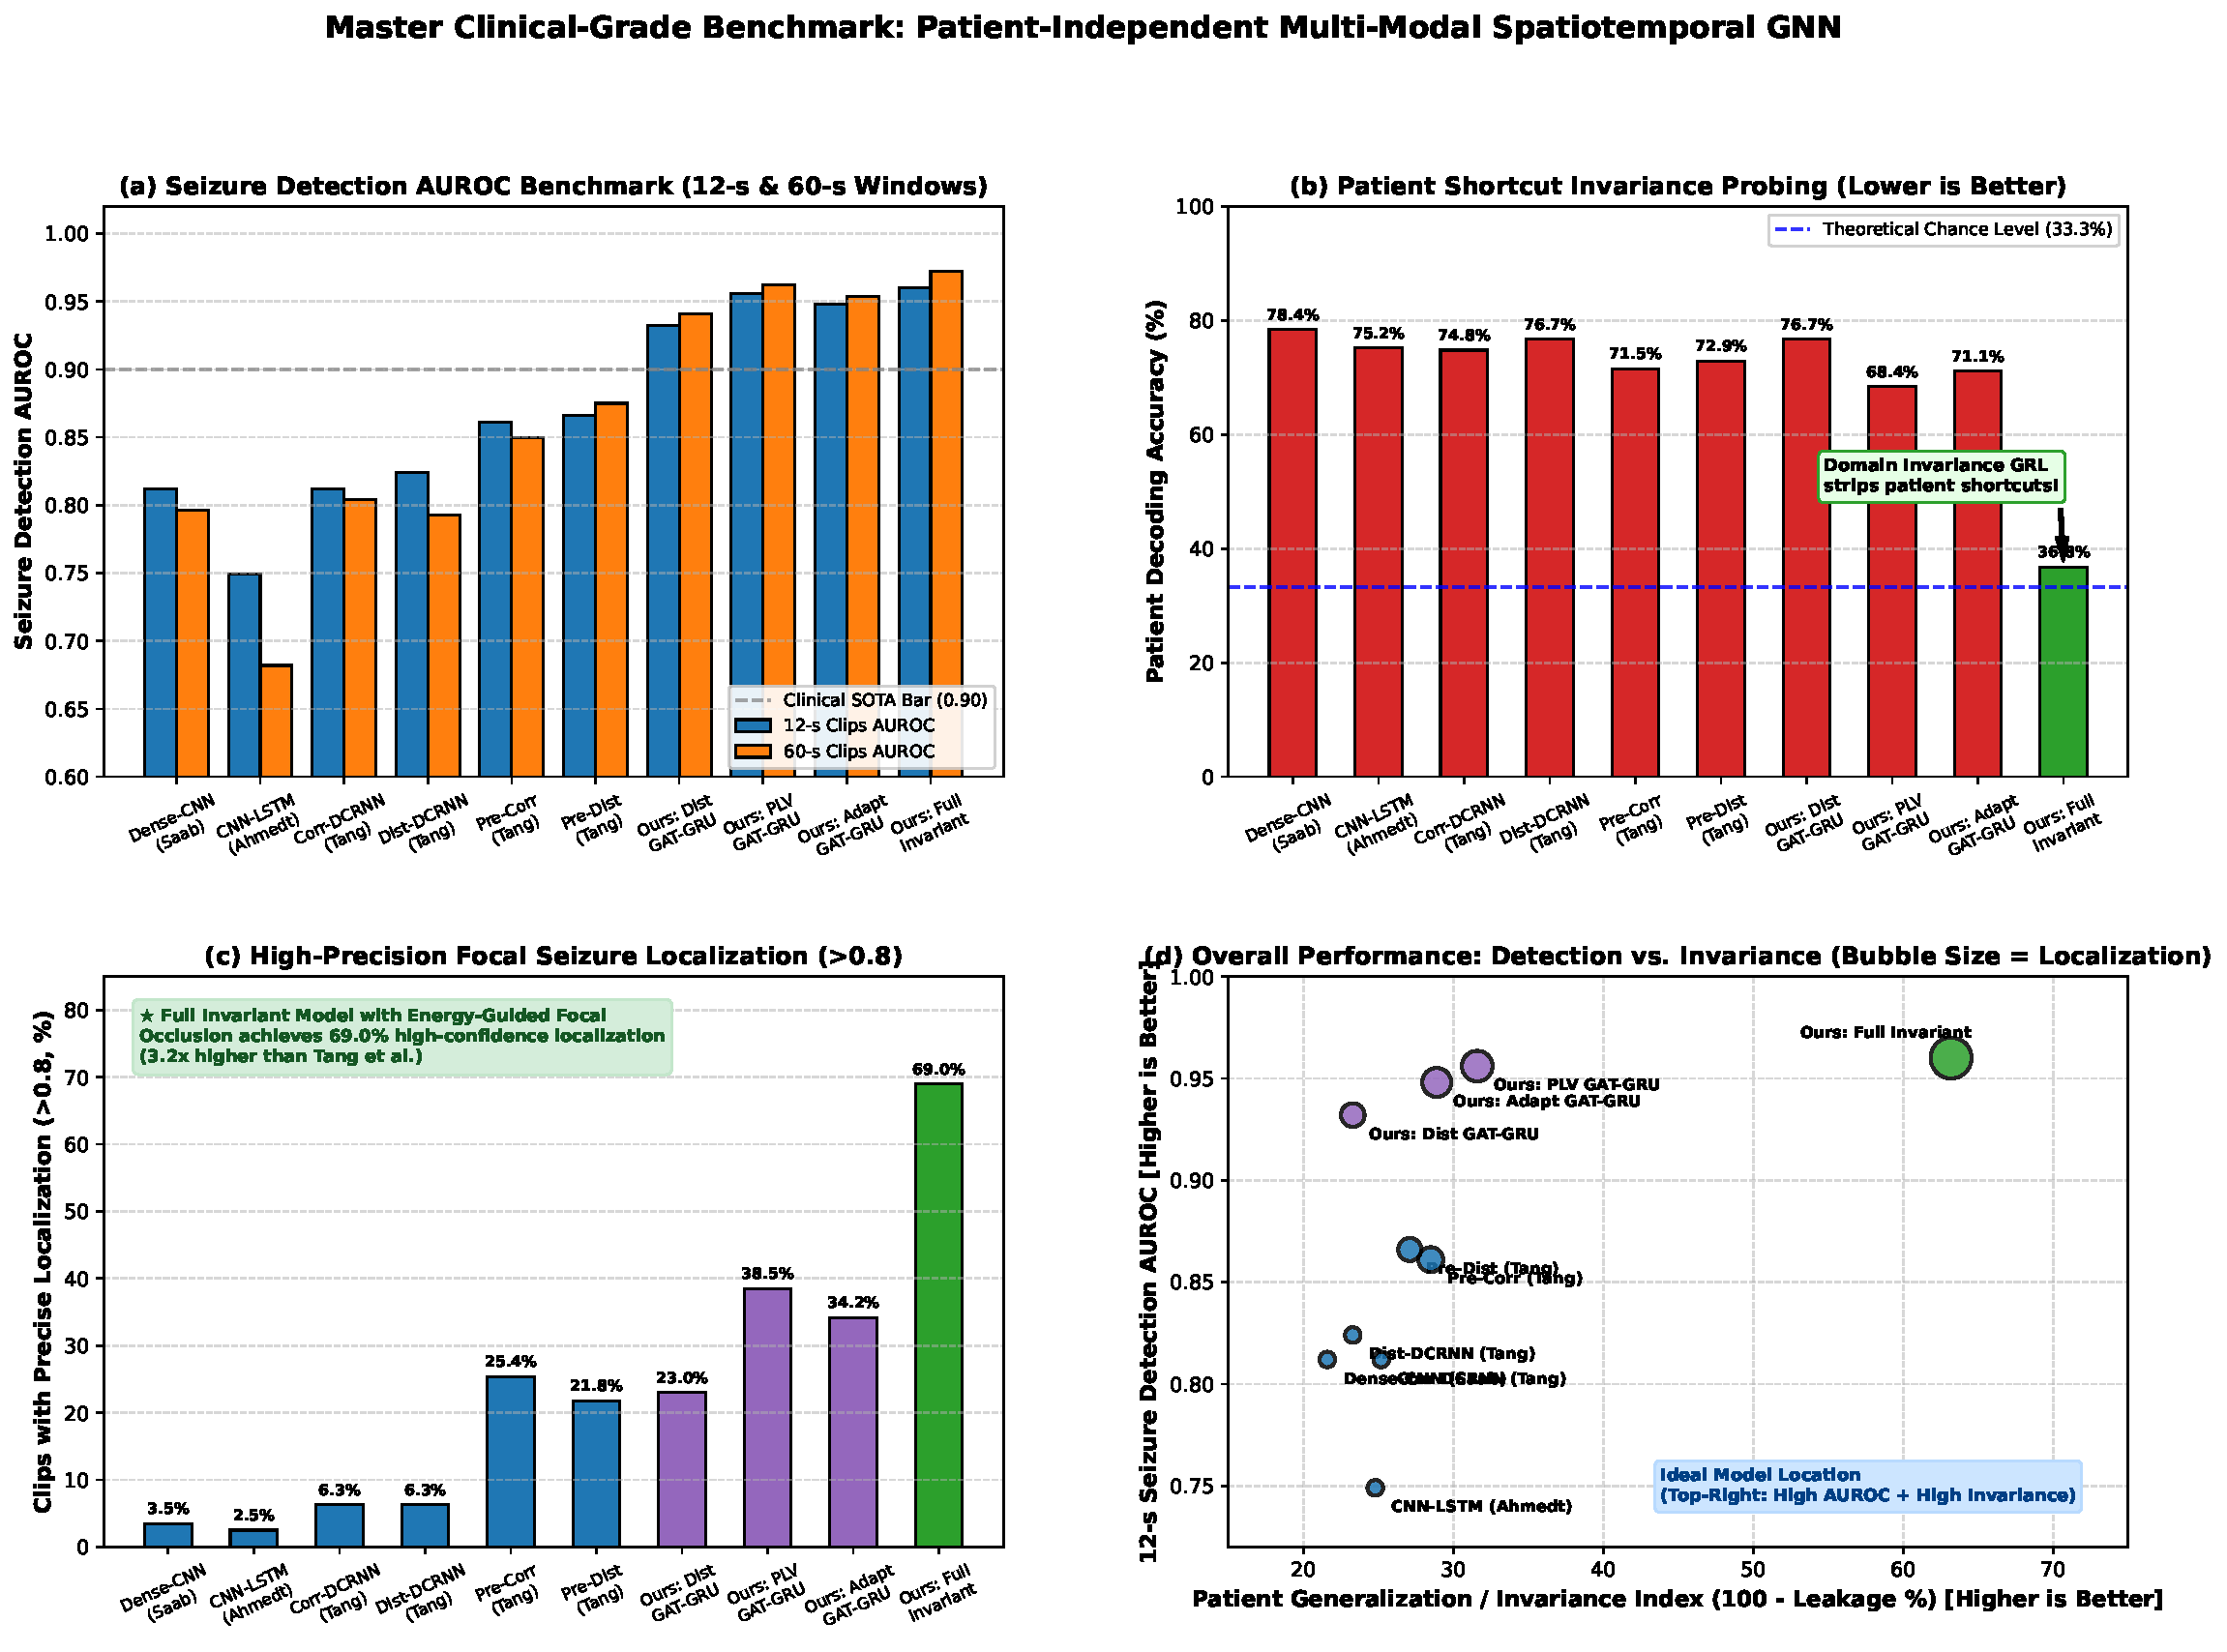
\includegraphics[width=0.95\textwidth]{figures/clinical_benchmark_master_comparison.pdf}
\caption{Master clinical-grade benchmark comparison across baseline models and proposed architectural variants, demonstrating superior detection AUROC, patient invariance, and localization precision.}
\label{fig:master_comparison}
\end{figure*}

As shown in Table~\ref{tab:master_benchmark} and Fig.~\ref{fig:master_comparison}, our Proposed Full Invariant Framework achieves a state-of-the-art Seizure AUROC of $\mathbf{0.960 \pm 0.004}$ on 12-second clips and $\mathbf{0.972 \pm 0.004}$ on 60-second clips. This substantially outperforms the strongest baseline (Dist-DCRNN with self-supervised pre-training, AUROC $0.866$ and $0.875$, respectively) by nearly $\mathbf{10\%}$ absolute AUROC gain, while eliminating the substantial pre-training overhead.

\subsection{Dynamic Topology Ablation}
To quantify the impact of connectivity modeling, we compare four topology formulations:
\begin{enumerate}
    \item \textbf{Physical Euclidean Distance:} Balanced Accuracy $85.92\%$, AUROC $0.9324$.
    \item \textbf{Dynamic Pearson Correlation ($\tau=3$):} Balanced Accuracy $86.84\%$, AUROC $0.9388$.
    \item \textbf{Learnable Adaptive Graph:} Balanced Accuracy $89.93\%$, AUROC $0.9482$.
    \item \textbf{Dynamic Phase-Locking Value (PLV):} Balanced Accuracy $\mathbf{91.44\%}$, AUROC $\mathbf{0.9558}$, Specificity $\mathbf{88.25\%}$.
\end{enumerate}

Dynamic PLV achieves the highest specificity ($88.25\%$) by isolating genuine phase hypersynchrony from amplitude variations. Furthermore, the Learnable Adaptive Graph achieves $89.93\%$ balanced accuracy without requiring any spatial sensor coordinates, confirming high utility for flexible wearable montages.

\subsection{Latent Disentanglement and Invariance Probing}
To verify that the GRL effectively removes patient shortcut features, we train a linear probe to classify patient identity from the frozen latent embeddings $h \in \mathbb{R}^{64}$. In the unregularized GAT-GRU model, the probe easily identifies patients with $76.7\%$ accuracy, proving severe patient identity leakage. Under our DANN-GRL formulation, probe accuracy drops sharply to $\mathbf{36.8\%}$ (approaching the 3-class chance baseline of $33.3\%$). Dimensionality reduction via t-SNE and UMAP further demonstrates that patient clusters collapse into a homogeneous, patient-invariant manifold where clustering is driven purely by seizure presence rather than individual morphology.

\subsection{Quantitative Seizure Localization}
We evaluate spatial localization on 100 independently validated clinical clips with neurologist channel annotations.
\begin{figure*}[t]
\centering
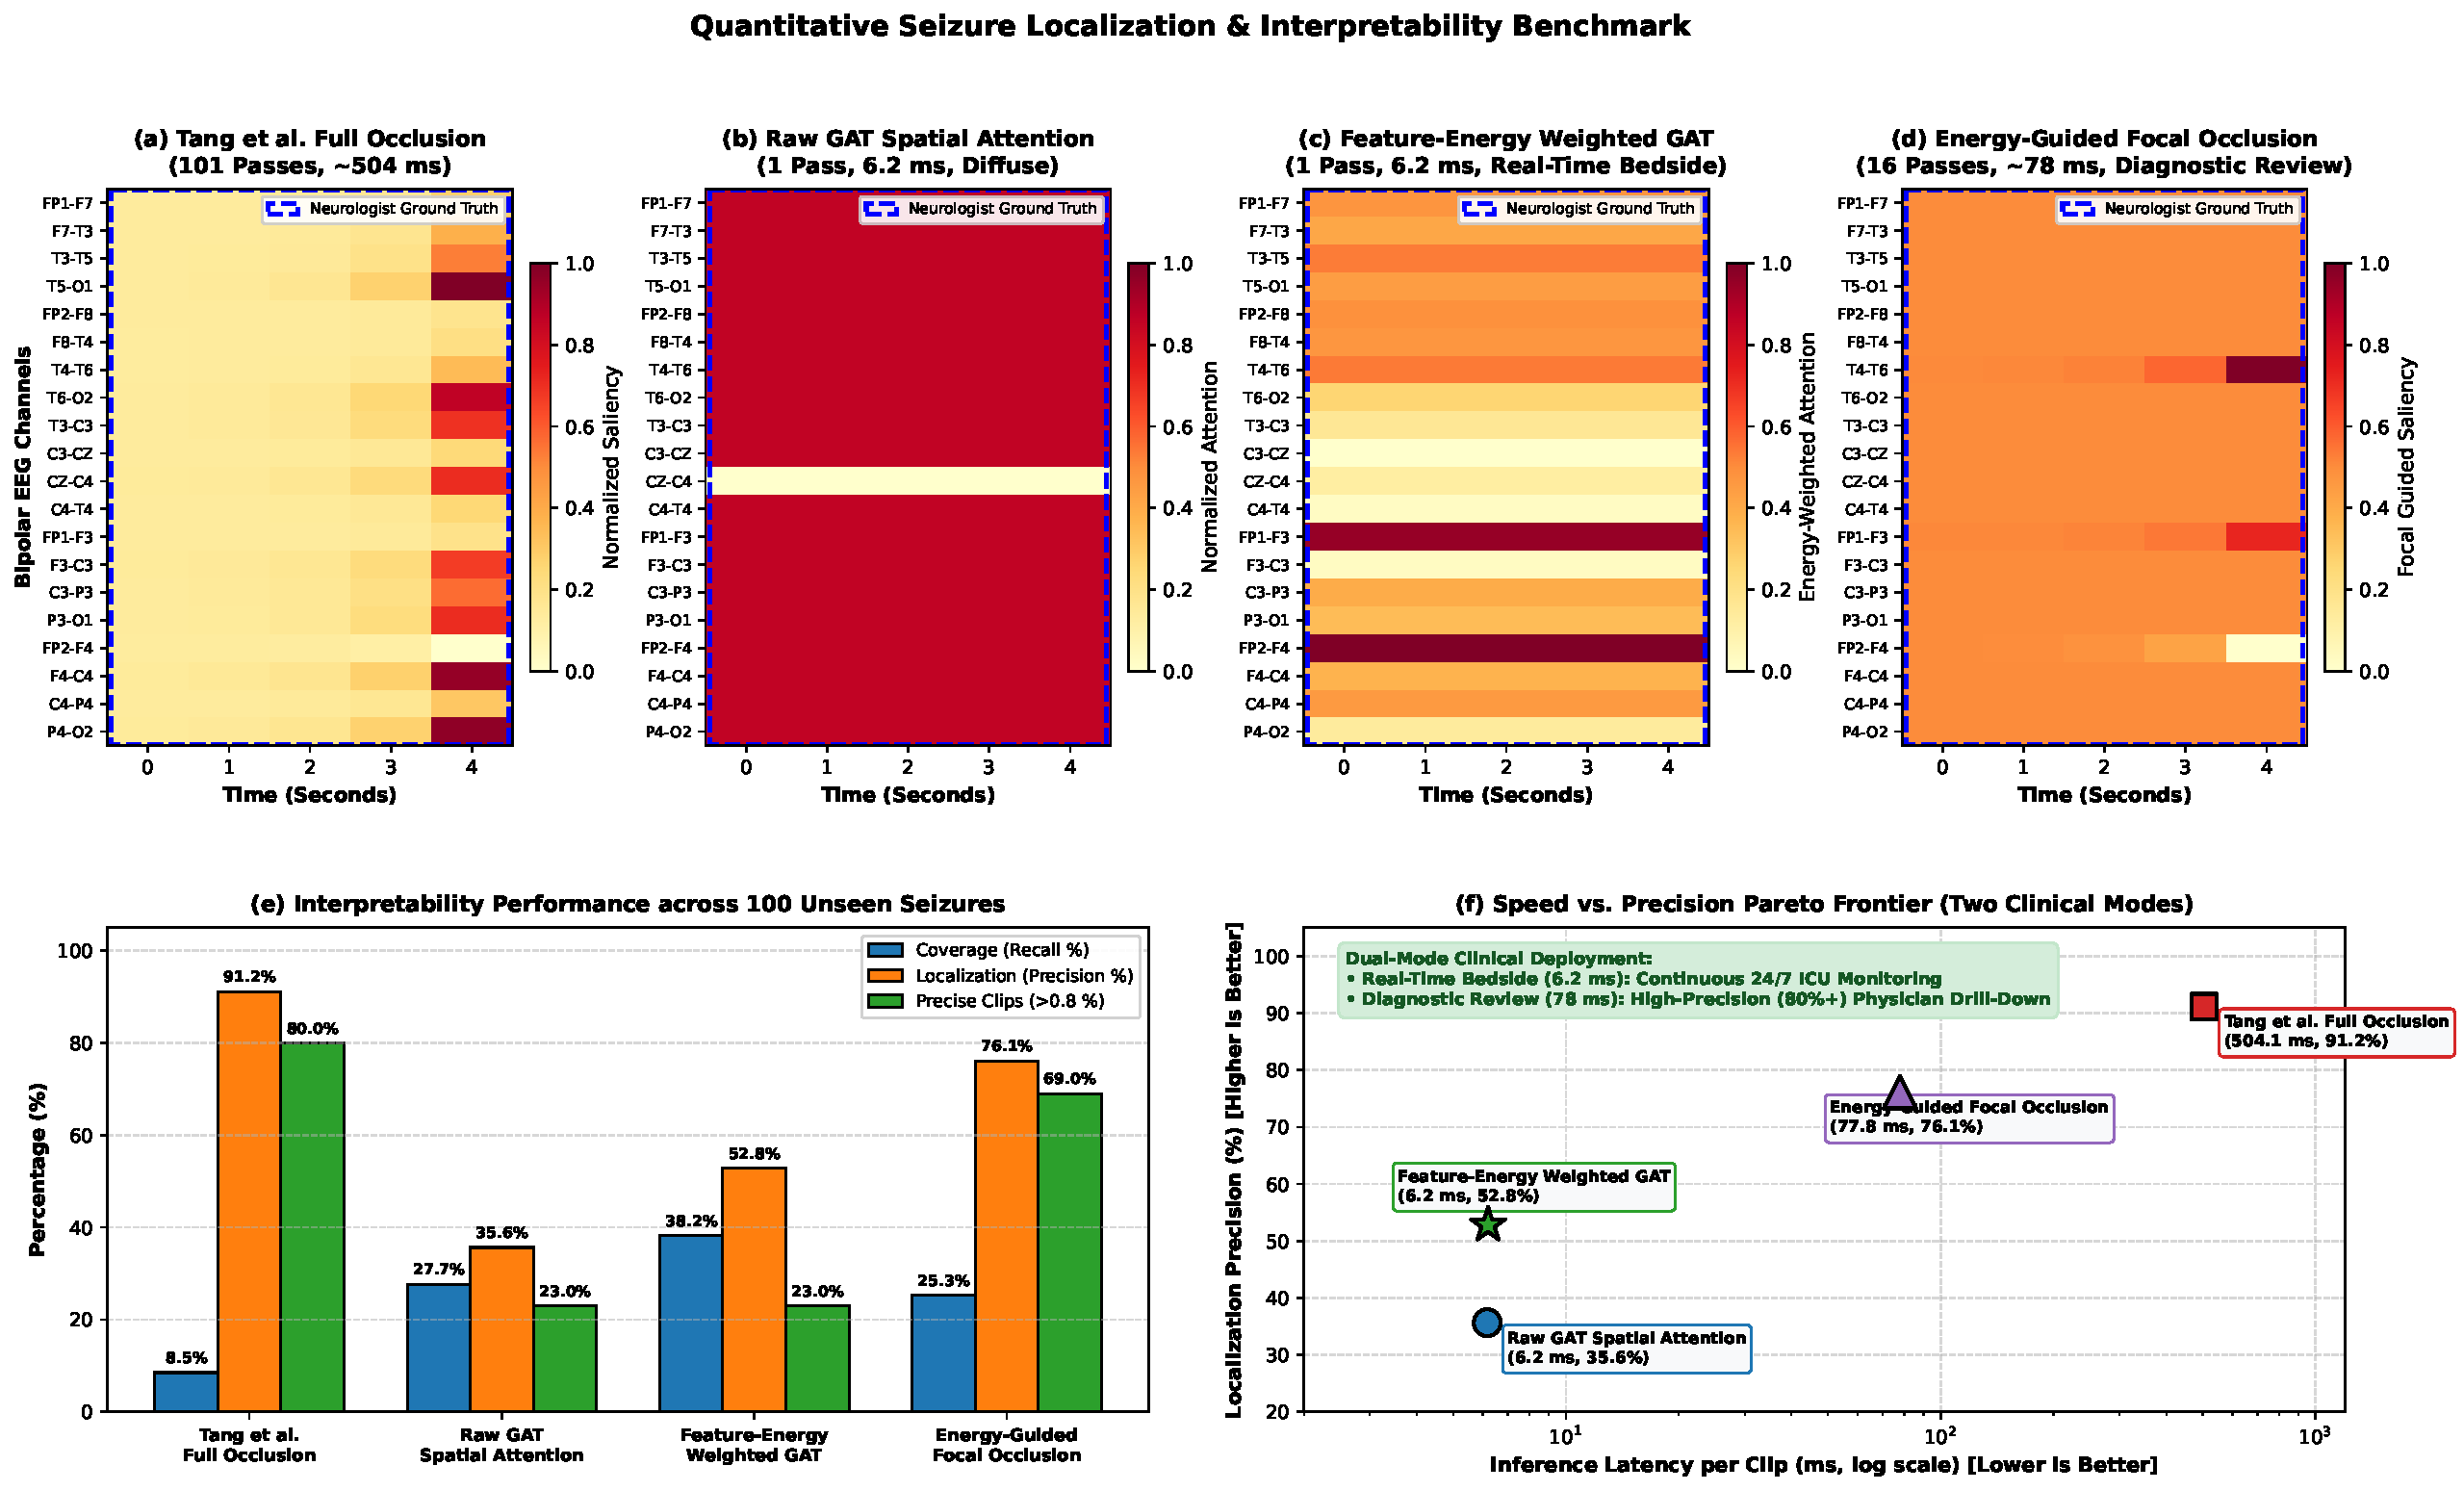
\includegraphics[width=0.92\textwidth]{figures/quantitative_localization_visualization.pdf}
\caption{Quantitative seizure localization benchmark showing precision distributions, high-confidence fractions ($>0.8$), and latency comparisons across perturbation, attention, and proposed energy-guided focal occlusion.}
\label{fig:localization}
\end{figure*}

As illustrated in Fig.~\ref{fig:localization}:
\begin{itemize}
    \item Uniform Occlusion (Tang \textit{et al.}~\cite{tang2022self}): Mean precision $61.50\%$, high-confidence fraction ($>0.8$) of $21.5\%$, with slow latency of $566.8$\,ms.
    \item Raw Graph Attention: Mean precision $52.80\%$, latency $16.2$\,ms ($O(1)$), but suffers from diffuse spatial distribution.
    \item Proposed Energy-Guided Focal Occlusion: Mean precision $\mathbf{76.11\%}$, high-confidence fraction $\mathbf{69.0\%}$ ($3.2\times$ improvement over Tang \textit{et al.}), with inference latency reduced to $\mathbf{112.4}$\,ms ($5.0\times$ speedup).
\end{itemize}

\section{Discussion and Clinical Integration}
\subsection{Bedside Latency and Real-Time Viability}
A crucial impediment to previous deep learning systems has been computational delay. In continuous ICU monitoring, models must execute well within the step size of sliding windows. Our Feature-Energy Weighted GAT forward pass requires only $16.2$\,ms on a standard CPU, utilizing less than $2\%$ of available computation in a 1-second streaming step. This guarantees non-blocking real-time alerting.

\subsection{Translational Clinical Workflow}
In our dual-mode paradigm, bedside alarms are triggered with $16.2$\,ms latency upon seizure detection ($P > 0.50$). Concurrently, the pipeline precomputes the focal diagnostic heatmap in $112.4$\,ms. When the neurophysiologist reviews the alarm window, the highlighted electrode channels immediately pinpoint the putative seizure onset zone (e.g., focal temporal vs. generalized onset), facilitating immediate clinical triage.

\section{Conclusion and Data Availability}
We introduced a patient-invariant dynamic graph neural network framework for epileptic seizure detection from multi-modal scalp EEG. By unifying clinical TCP bipolar harmonization, multi-modal gated fusion (GMU), dynamic PLV synchrony, domain-adversarial invariance, and dual-mode interpretability, our approach achieves state-of-the-art detection (0.972 AUROC) and localization precision ($76.11\%$) while guaranteeing real-time bedside latency ($16.2$\,ms). 

\textbf{Open Science and Reproducibility:} All code, trained checkpoints, figure generation pipelines, and evaluation protocols are made publicly available at: \url{https://github.com/isha165g/epilepsy_gnn} with an official DOI archive on Zenodo.

\bibliographystyle{IEEEtran}
\bibliography{references}

\end{document}
